\chapter{Gas and wave dark matter}\label{ch:hydro-wavedm}
\chapterstatus{written}{2026-11-14}

Besides collisionless particles \fml{} has three solvers for other kinds of matter: a finite-volume Euler solver for
an ideal gas on a uniform mesh, smoothed-particle hydrodynamics (SPH) for adiabatic gas, and a spectral
Schr\"odinger--Poisson solver for wave (fuzzy) dark matter. All three run serially or with slab MPI and OpenMP, take
external gravity through callbacks and support a prescribed cosmological expansion. They are libraries: none is yet
an evolution mode of SimulationCode.

\begin{modulebox}{Hydrodynamics, SPH, WaveDarkMatter}
\file{Hydrodynamics} (namespace \nsp{FML::HYDRODYNAMICS}): \file{EquationOfState.h} (\cls{IdealGas}, shared with SPH),
\file{Euler.h} (states and fluxes), \file{Riemann.h}, \file{ExactRiemann.h}, \file{FiniteVolume.h},
\file{CartesianGrid.h}.\par
\file{SPH} (namespace \nsp{FML::SPH}): \file{SPH.h} (\cls{Solver}), \file{Kernel.h}, \file{Cells.h}, \file{Transport.h}.\par
\file{WaveDarkMatter} (namespace \nsp{FML::WAVEDM}): \file{SchrodingerPoisson.h} (\cls{Solver}, \cls{Physics}),
\file{WaveGrid.h}, \file{TimeFactors.h}, \file{Checkpoint.h}.\par
Documentation: the module READMEs and \file{tests/RESULTS.md} of each.
\end{modulebox}

\section{Finite-volume hydrodynamics}\label{sec:hydro-fv}

\paragraph*{Equations.} The Euler equations of an ideal gas with $P=(\gamma-1)\rho u$,
\begin{equation}
\partial_t\bm U+\nabla\cdot\bm F(\bm U)=\bm S,\qquad
\bm U=\begin{pmatrix}\rho\\ \rho\bm v\\ E\end{pmatrix},\quad
\bm F=\begin{pmatrix}\rho\bm v\\ \rho\bm v\otimes\bm v+P\,\mathbb I\\ (E+P)\bm v\end{pmatrix},\quad
E=\rho u+\tfrac12\rho v^2,
\end{equation}
are solved on a uniform Cartesian mesh in 1D, 2D or 3D (\cls{FiniteVolume}). \code{Primitive<D>} holds
$(\rho,\bm v,P)$; \code{Conserved<D>} holds $(\rho,\rho\bm v,E,\rho u_{\rm aux})$, the last an auxiliary advected
internal-energy density for the dual-energy option.

\paragraph*{Riemann solvers.} The interface flux comes from an approximate Riemann solver (\code{riemann(left, right,
eos, axis, method)}):
\begin{itemize}
\item \emph{Rusanov}: the local Lax--Friedrichs flux with the largest $|v_n|+c$ of the two states;
\item \emph{HLLE} \cite{Harten1983,Einfeldt1988}: the HLL flux with Roe/Einfeldt wave-speed bounds widened to include
      both sound cones;
\item \emph{HLLC} \cite{Toro1994}: restores the contact wave and preserves tangential contact states; it falls back to
      HLLE for generated vacuum or degenerate and non-positive star states.
\end{itemize}
The result reports the flux, interface velocity, maximum signal speed, the method actually used and a fallback reason.
\cls{ExactRiemann} solves the pressure-matching equation of the exact ideal-gas Riemann problem (bracketed solve in
$\ln P$) and samples shocks, contacts, rarefaction fans and generated vacuum; it is the independent reference of the
tests.

\paragraph*{Discretisation.} The directional flux divergences are summed in one unsplit method-of-lines right-hand
side. Second order uses componentwise primitive linear reconstruction with generalised minmod/MC slopes
($\theta\in[1,2]$, default 1.5); the time integrator is SSPRK2. A non-physical reconstruction is reset to the cell
state (evolved densities and pressures are never clipped). Each forward-Euler trial is checked collectively; a failed
high-order trial is recomputed with first-order Rusanov fluxes everywhere, and \code{advance(max_dt)} then halves the
step if needed. The time step is a global unsplit CFL bound plus expansion and gravity limits. There is no density,
pressure or temperature floor.

\paragraph*{Dual energy.} For high Mach numbers $\rho u_{\rm aux}$ is evolved with its own advective flux and
pressure-work source; when $(E-K)/E$ falls below \code{pressure_threshold} ($10^{-3}$) the pressure is taken from it and
$E$ reset to $K+\rho u_{\rm aux}$, a non-conservative correction recorded in an energy-repair ledger.

\paragraph*{Boundaries and parallelism.} Periodic, zero-gradient outflow or reflecting boundaries per dimension; two
halo layers. Integer $x$ slabs $[\lfloor rN_x/P\rfloor,\lfloor(r+1)N_x/P\rfloor)$ (empty ranks allowed), halo planes
routed to their owners in bounded chunks.

\paragraph*{Gravity and expansion.} A collective \code{Gravity} callback supplies the peculiar acceleration $\bm g$;
momentum gets $\rho\bm g$ and energy $\bm m\cdot\bm g$. In 3D a prescribed background $a(t)$, $H$ makes lengths
comoving, velocities physical peculiar velocities, $\rho_c=a^3\rho$ and $P_c=a^3P$; spatial divergences carry $1/a$, the
momentum source is $-H\bm m+\rho_c\bm g$ and the energy source $\bm m\cdot\bm g-2HK-3HP_c$.

\begin{cppcode}[A Sod shock tube]
#include <FML/Hydrodynamics/FiniteVolume.h>
namespace H = FML::HYDRODYNAMICS;
H::Options<1> options;
options.shape = {256}; options.lengths = {1}; options.gamma = 1.4;
options.boundaries = {{{H::Boundary::Outflow, H::Boundary::Outflow}}};
H::FiniteVolume<1> gas(options, [](const auto & x) {
    return x[0] < .5 ? H::Primitive<1>{1, {0}, 1} : H::Primitive<1>{.125, {0}, .1};
});
while (gas.time() < .2) gas.advance(.2 - gas.time());
auto totals = gas.diagnostics();        // mass, momentum, energy (collective)
\end{cppcode}

\begin{validation}[Validation: finite volume (\file{Hydrodynamics/tests/RESULTS.md})]
\begin{itemize}
\item Smooth problems: observed orders 2.10 (1D advection), 1.74 (2D), 1.50 (3D at $16\to32$), 2.10 (linear sound).
\item Shock tubes against the exact solver: Sod density L1 errors $3.5\times10^{-3}$, $1.7\times10^{-3}$,
      $1.1\times10^{-3}$ at 128, 256, 512 cells; Lax, strong shock, two rarefactions and generated vacuum.
\item Mass and total energy conserved to round-off in 2D/3D blasts; identical results on 1, 2 and 4 ranks; dual energy
      retains the temperature in high-Mach advection.
\end{itemize}
\end{validation}

\begin{figure}[htbp]
\centering
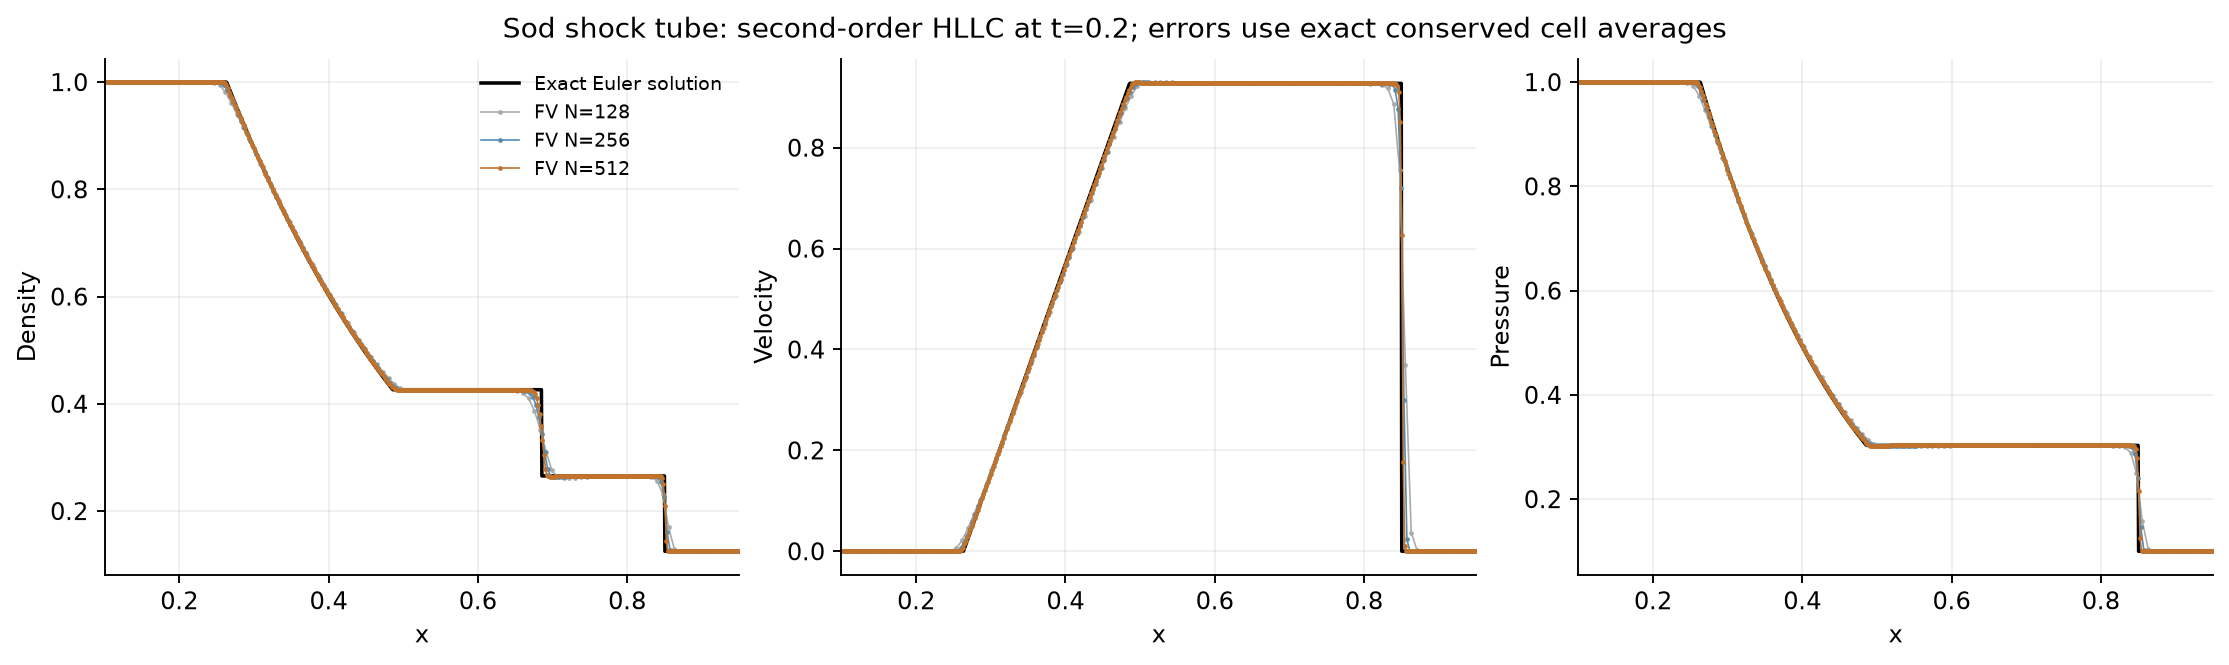
\includegraphics[width=\textwidth]{hydro_fv_sod}\\[2mm]
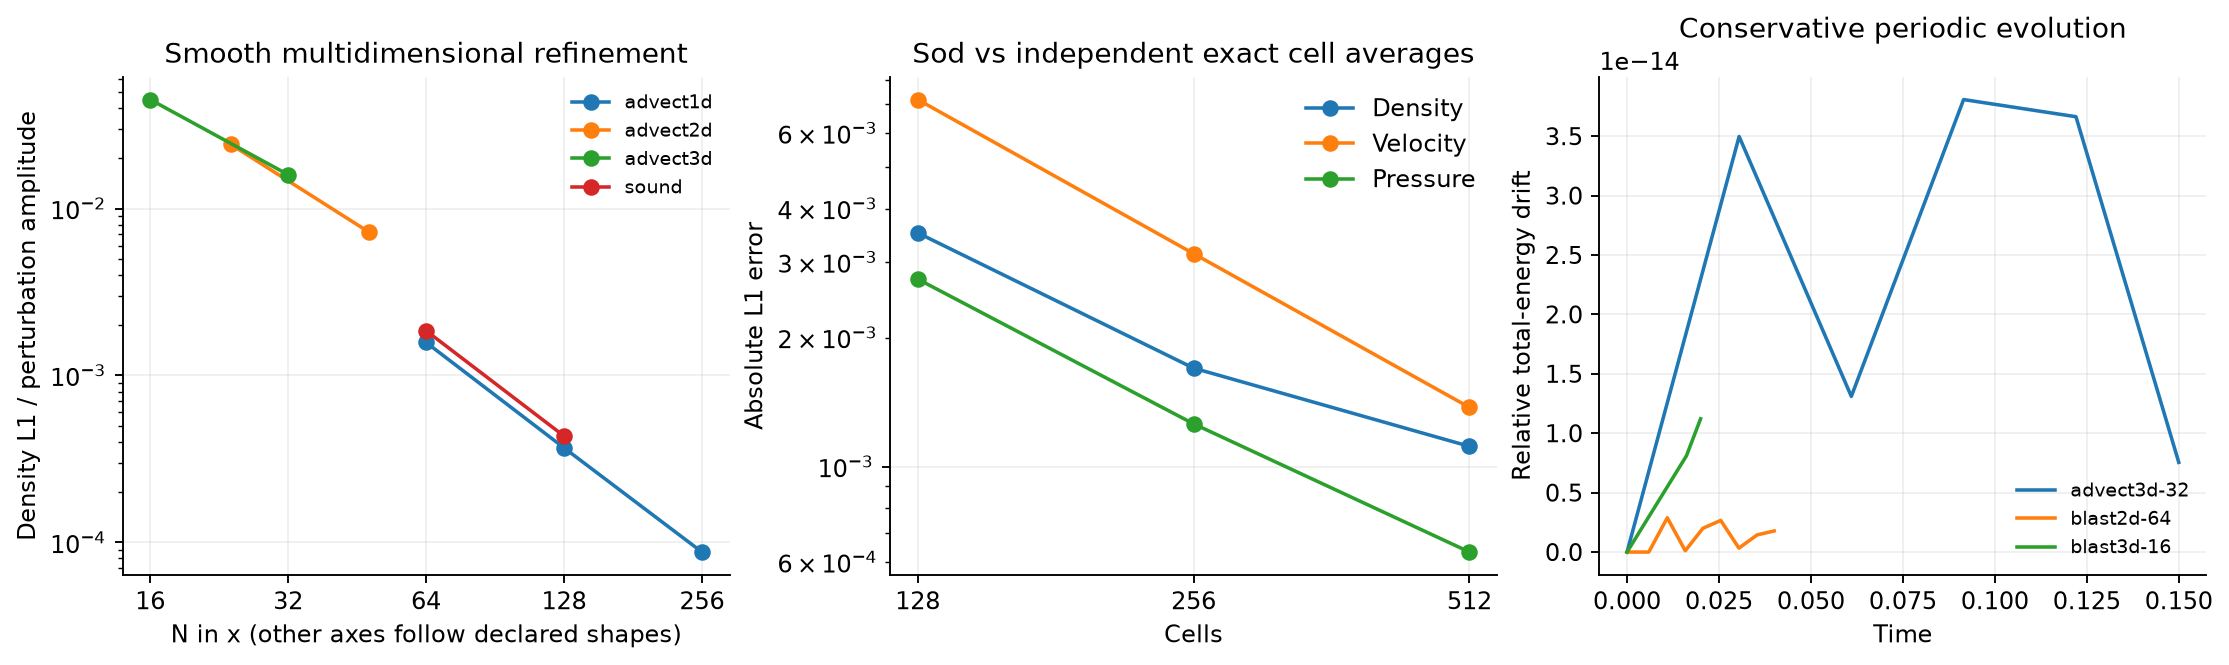
\includegraphics[width=\textwidth]{hydro_fv_convergence}
\caption{Finite-volume validation (\file{Hydrodynamics/tests/figures}). \emph{Top:} the Sod shock tube with second-order HLLC at
$t=0.2$ for 128, 256 and 512 cells against the exact Euler solution. \emph{Bottom:} convergence of smooth advection and sound waves in
1--3D, the Sod L1 errors against exact cell averages, and the relative drift of the total energy in periodic runs ($\lesssim4\times10^{-14}$).}
\label{fig:hydro-fv}
\end{figure}


\section{Smoothed-particle hydrodynamics}\label{sec:hydro-sph}

\cls{Solver} evolves periodic gas particles in 1D/2D/3D with the variational density--energy formulation summarised by
Price \cite{Price2012}. The kernel is the cubic B-spline $W=\sigma_Dh^{-D}f(r/h)$ with support $2h$,
$f=1-\frac32q^2+\frac34q^3$ for $q<1$ and $\frac14(2-q)^3$ for $1\le q<2$ ($\sigma_D=\frac23,\frac{10}{7\pi},\frac1\pi$).
Each particle solves for its smoothing length and density together, and the forces follow from the Lagrangian:
\begin{gather}
\rho_i=\sum_jm_jW(r_{ij},h_i),\qquad h_i^D\rho_i=\eta^Dm_i,\qquad
\Omega_i=1+\frac{h_i}{D\rho_i}\sum_jm_j\frac{\partial W(r_{ij},h_i)}{\partial h_i},\\
\frac{\dd\bm v_i}{\dd t}=-\sum_jm_j\left[\frac{P_i}{\Omega_i\rho_i^2}\nabla_iW(h_i)+\frac{P_j}{\Omega_j\rho_j^2}\nabla_iW(h_j)
+\Pi_{ij}\nabla_i\bar W\right],\\
\frac{\dd u_i}{\dd t}=\sum_jm_j\left[\frac{P_i}{\Omega_i\rho_i^2}\bm v_{ij}\cdot\nabla_iW(h_i)+\tfrac12\Pi_{ij}\bm v_{ij}\cdot\nabla_i\bar W\right].
\end{gather}
The $\Omega$ (grad-$h$) terms make the equations exactly conservative; force searches use the union of both particles'
supports. The $(h,\rho)$ root is found by bracketed Newton/bisection within $[h_{\min},h_{\max}]$ (a failure is a
collective error, never a silent clamp).

\paragraph*{Dissipation.} Artificial viscosity for approaching pairs,
$\mu_{ij}=\bar h\,\bm v_{ij}\cdot\bm r_{ij}/(r^2+\epsilon\bar h^2)$,
$\Pi_{ij}=(-\alpha\bar c\mu_{ij}+\beta\mu_{ij}^2)/\bar\rho$ (default $\alpha=1$, $\beta=2$), with the Balsara shear limiter
$|\nabla\cdot\bm v|/(|\nabla\cdot\bm v|+|\nabla\times\bm v|+\epsilon c/h)$ \cite{Balsara1995}; optional artificial
conductivity $\alpha_u\sum_jm_j(u_i-u_j)\sqrt{|P_i-P_j|/\bar\rho}\,\bar W'/\bar\rho$.

\paragraph*{Time integration and cosmology.} A global time step (Courant, acceleration and energy-change limits) with
Heun RK2; a failed step restores the particles. An \code{ExternalForce} callback adds gravity. With a prescribed 3D
background, positions and $h$ are comoving and
\begin{equation}
\frac{\dd\vx}{\dd t}=\frac{\bm v}{a},\qquad
\frac{\dd\bm v}{\dd t}=\frac{\bm a_{\rm hydro}}{a}-H\bm v+\bm g,\qquad
\frac{\dd u}{\dd t}=\frac{\dot u_{\rm hydro}}{a}-3(\gamma-1)Hu,
\end{equation}
with the physical relative velocity $\bm v_{ij}+aH\bm x_{ij}$ in the viscosity. MPI uses the $x$ slabs of \fml{} with
ghost exchanges within $2h_{\max}$ for densities and twice the largest $h$ for forces.

\begin{validation}[Validation: SPH (\file{SPH/tests/RESULTS.md})]
Densities, $\Omega$, forces and heating against all-pair sums ($10^{-15}$); total momentum and energy rates conserved to
$10^{-16}$; the forces equal the fixed-entropy derivative of the internal energy ($2\times10^{-10}$); sound waves
converge at second order in 1D; Sod shock tube L1 density errors $0.017$, $0.009$, $0.005$ for 225, 450, 900 particles
with gas-energy drift $\sim10^{-6}$; uniform expansion reproduces $v\propto a^{-1}$ and $u\propto a^{-2}$; identical results on
1, 2 and 4 ranks.
\end{validation}

\begin{figure}[htbp]
\centering
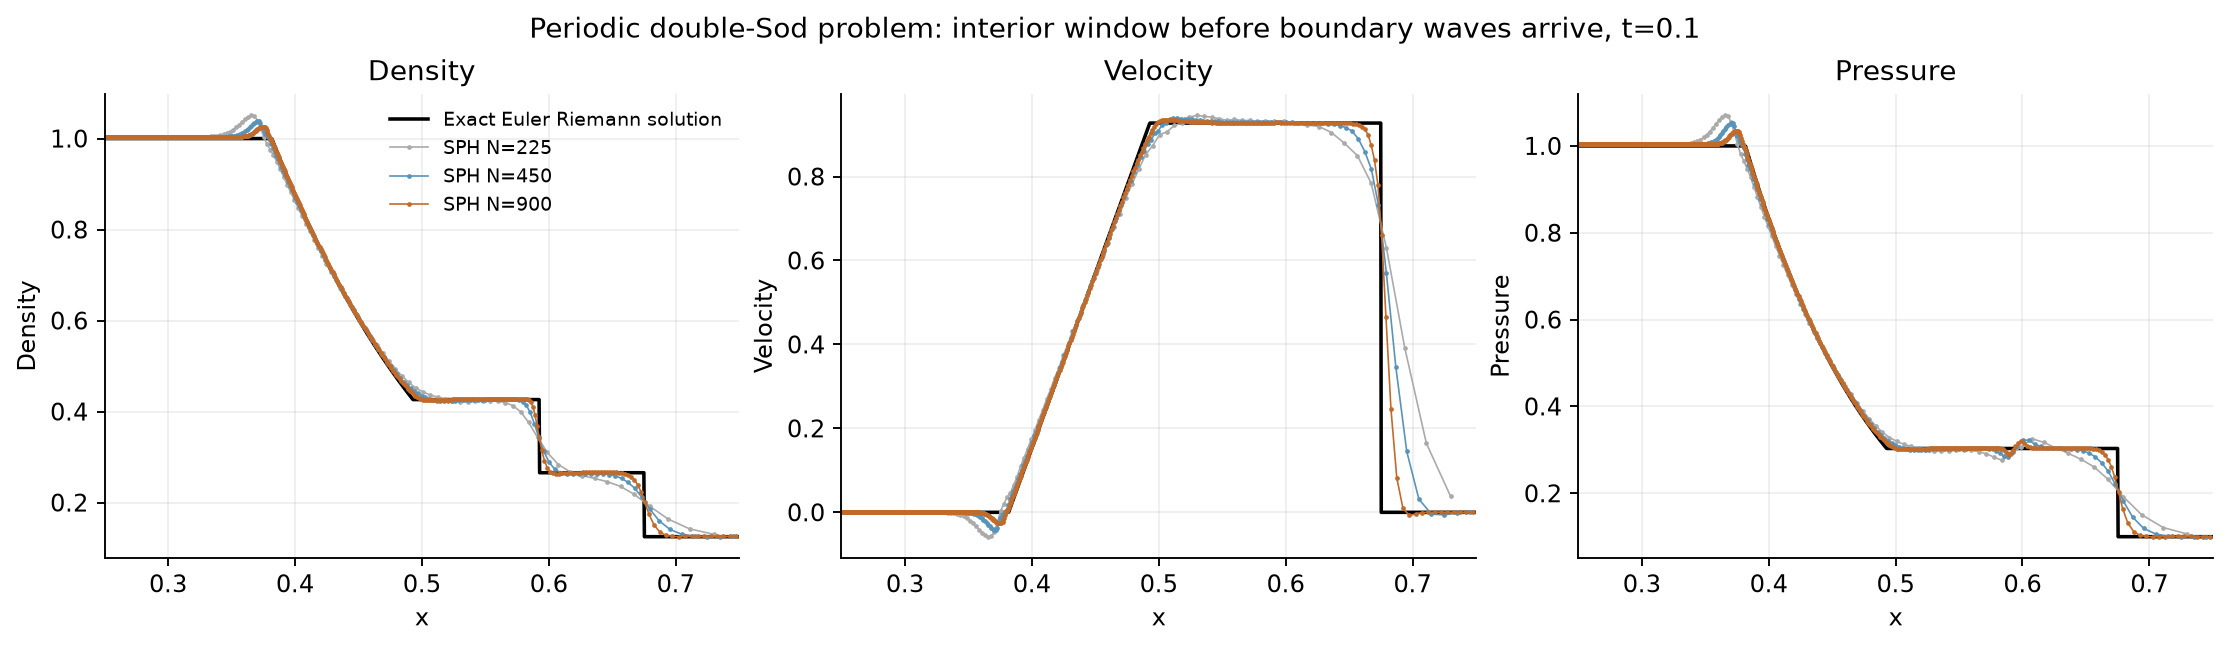
\includegraphics[width=\textwidth]{sph_sod}
\caption{SPH on the periodic double-Sod problem at $t=0.1$ for 225, 450 and 900 particles against the exact Riemann solution
(\file{SPH/tests/figures}): the blips at the contact discontinuity and the smoothed shock are the usual SPH behaviour and shrink with
resolution.}
\label{fig:sph-sod}
\end{figure}


\section{Wave dark matter}\label{sec:wavedm}

Ultralight bosons of mass $m$ ($\sim10^{-22}$\,eV) have a de Broglie wavelength of astrophysical size and are described
by a classical wave obeying the Schr\"odinger--Poisson equations \cite{Hu2000FDM,Schive2014}. With $\eta=\hbar/m$ and the
comoving wavefunction $\psi$ (the homogeneous $a^{-3/2}$ dilution absorbed), $\rho_{\rm com}=|\psi|^2$ and $U=a\Phi$,
\begin{equation}
i\frac{\partial\psi}{\partial t}=-\frac{\eta}{2a^2}\nabla^2\psi+\frac{U}{\eta a}\psi,\qquad
\nabla^2U=4\pi G\left(\rho_{\rm com}+\rho_{\rm ext}-\bar\rho_{\rm tot}\right),
\end{equation}
in cosmic time, for one non-relativistic species without self-interaction. \code{Physics::from_si(m_eV, L0, T0, M0)}
converts to code units ($\eta=(\hbar/m)T_0/L_0^2$, $G=G_{\rm SI}M_0T_0^2/L_0^3$).

\paragraph*{Split-step method.} The wavefunction lives on a full complex grid (\cls{CFFTWGrid} slabs or
\cls{CPencilGrid} pencils; all $N^3$ modes are independent). A step is the kick--drift--kick split
\begin{equation}
\psi\leftarrow e^{-iU_{\rm init}B/(2\eta)}\psi,\qquad
\psi_{\vk}\leftarrow e^{-i\eta k^2A/2}\psi_{\vk},\qquad
\psi\leftarrow e^{-iU_{\rm final}B/(2\eta)}\psi,\qquad A=\int\frac{\dd t}{a^2},\quad B=\int\frac{\dd t}{a},
\end{equation}
with the potential recomputed from the density after the kinetic substep (the potential substeps preserve the
density exactly). At fixed $a$ this is the second-order Strang split; with the integrated factors it is second order for
a smooth prescribed expansion. \code{step_scale_factor(a_next, H)} computes $\dd t=\int\dd a/(aH)$, $A$ and $B$ by
Gauss--Legendre quadrature. The kinetic phase is a product of three tabulated 1D factors; a self-gravitating step costs
four complex FFTs. \code{suggested_timestep} bounds the kinetic and potential phases per step. No norm repair or high-$k$
filtering is applied.

\paragraph*{Initial conditions and coupling.} \code{initialize(field)}, \code{initialize_density_phase(rho, theta)}
($\psi=\sqrt\rho\,e^{i\theta}$) or \code{initialize_density_velocity_potential(rho, sigma)} ($\theta=a\sigma/\eta$ for
$\bm u=\nabla\sigma$, single stream). An external comoving density (e.g.\ CDM particles) can source the potential
(\code{set_external_density}), and \code{gravity_acceleration} returns $-\nabla U/a^3$ for particles.

\paragraph*{Energy diagnostics.} $K=\frac{\eta^2}{2a^2}\int|\nabla\psi|^2$, $W=\frac{1}{2a}\int\rho U$; in an expanding
background $\dd E/\dd t=-H(2K+W)$, and \cls{EnergyBalance} tracks the residual
$E(a)-E(a_0)+\int(2K+W)\,\dd\ln a$.

\begin{cppcode}[A wave dark matter run]
#include <FML/WaveDarkMatter/SchrodingerPoisson.h>
using namespace FML::WAVEDM;
auto physics = Physics::from_si(1e-22, FML::UTILS::SI::kpc, FML::UTILS::SI::Gyr, 1e7 * FML::UTILS::SI::Msun);
Solver solver(64, 20.0, physics);                  // 64^3, box of 20 code lengths
solver.initialize_density_phase([](auto x) { return 1.0 + 0.01 * std::cos(2 * M_PI * x[0] / 20.0); },
                                [](auto) { return 0.0; });
solver.step(1e-3);                                 // fixed a; or step_scale_factor(a_next, H)
auto d = solver.diagnostics();                     // mass, K, W, high-k tail fraction
\end{cppcode}

\begin{validation}[Validation: wave dark matter (\file{WaveDarkMatter/tests/RESULTS.md})]
Complex FFTs against explicit DFTs; free-wave dispersion, interference, Parseval, Poisson signs; a nonlinear $4^3$
field against an adaptive DOP853 method-of-lines reference; second-order convergence in $\Delta t$ (field errors
$1.7\times10^{-3}$, $4.3\times10^{-4}$, $1.1\times10^{-4}$ for $\Delta t=0.1$, $0.05$, $0.025$); a soliton from an
independent boundary-value solution stays stationary (relative static-energy drift $5\times10^{-8}$); slabs and
pencils agree to $10^{-14}$; versioned checksummed checkpoints restart with a different number of tasks.
\end{validation}
